\documentclass[11pt]{report}
% Seboholi Mamello (2022)

% Packages
\usepackage{amsmath}
\usepackage[a4paper]{geometry}
\usepackage{fullpage}
\usepackage{charter}
\usepackage{dirtytalk}
\usepackage{graphicx}
\usepackage{parskip}
\usepackage{pdfpages}

% Referencing
\usepackage[]{hyperref}
\hypersetup{
  colorlinks = true,
  urlcolor = blue,
  linkcolor = blue,
  citecolor = blue
}

% University of the Witwatersrand Citation Style
\usepackage{natbib} % Force natbib.sty to put citation labels in the reference list
\makeatletter
\renewcommand\NAT@biblabel[1]{\def\citeauthoryear##1##2{##1 ##2}[#1]\hfill}
\renewcommand\NAT@bibsetup[1]{%
  \setlength{\itemsep}{\bibsep}\setlength{\parsep}{\z@}}
\def\@lbibitem[#1]#2{%
  \if\relax\@extra@b@citeb\relax\else
    \@ifundefined{br@#2\@extra@b@citeb}{}{%
     \@namedef{br@#2}{\@nameuse{br@#2\@extra@b@citeb}}}\fi
   \@ifundefined{b@#2\@extra@b@citeb}{\def\NAT@num{}}{\NAT@parse{#2}}%
   \item[\hfil\hyper@natanchorstart{#2\@extra@b@citeb}\@biblabel{#1}%
    \hyper@natanchorend]%
    \NAT@ifcmd#1(@)(@)\@nil{#2}}
\makeatother


\bibliographystyle{named-wits}
\bibpunct{[}{]}{;}{a}{}{}  % to get correct punctuation for bibliography
\setlength{\skip\footins}{1.5cm}
\newcommand{\citets}[1]{\citeauthor{#1}'s \citeyearpar{#1}}
\renewcommand\bibname{References} 

\pagestyle{headings}

\pagestyle{plain}
\pagenumbering{arabic}

% Document
\begin{document}
\onecolumn
\thispagestyle{empty}

\
\begin{center}
    \vfill
    \LARGE BSc Hons: Computer Science\\[10pt]
    \LARGE Literature Review\\[30pt]
    \LARGE \textbf{Reinforcement Learning}\\[10pt]
    \LARGE Goal Selection Strategies for Learning Goal-Oriented Value Functions\\
    \vfill
    
\includegraphics[width=7.5cm]{images/wits-logo.png}
    \vfill
    \Large Mamello Seboholi\\
    \Large 1851317\\[10pt]
    \Large Supervised by Steven James\\
    \vfill
\end{center}

\chapter{Introduction}
The aim of this project is to extend the Goal-oriented Q-learning algorithm used in logical composition reinforcement 
learning (RL) by considering different use cases.

\chapter{Background and Related Work}

\section{Introduction}
This chapter serves to present our findings in related work to this paper. The paper has the following layout: section 
\ref{composition} explores knowledge transfer through composition with the focus on concurrent composition; and section 
\ref{conclusion} will serve as a conclusion for this chapter.

\section{Composition} \label{composition}
It is essential that we discuss the idea of $composition$ \citep{todorov2009compositionality} within the context of 
this project as we aim to improve on the literature focused on this topic.

\citet{nangue2020boolean} discusses the need for reinforcement learning (RL) agents to have an ability of knowledge 
transfer as reinforcement learning (RL) problems become expensive. The paper models tasks using Markov Decision Processes
(MDPs) where an MDP is defined as a quadruple (4-tuple) composed of the (i) state space $S$, (ii) action space $A$, (iii)
Markov kernel defined by $\rho$ that takes $S\times A$ to $S$, and (iv) reward function $r$ that has real values and 
bounded by a minimum and maximum $r$ values.

RL agent's goal is to work out a policy $\pi$ that maps $S$ to $A$, which solves a given task optimally. Extended reward 
function and extended Q-value functions are defined. Tasks, as well as the extended Q-value functions are defined 
as Boolean algebra.

This paper, along with \citet{todorov2009compositionality}, \citet{saxe2017hierarchy}, \citet{haarnoja2018composable}, 
\citet{van2019composing}, \citet{hunt2019composing}, and \citet{peng2019mcp} focus on concurrent composition, where 
novel tasks are formed by combining previously learned tasks. Another group of literature focus on sequentially chaining 
learned policies to solve complex tasks, examples of this is options \citep{sutton1999between} and hierarchical 
reinforcement learning \citep{barto2003recent}.

This paper is the basis for this project with the focus being on how agents choose between maximizing goals and 
discovering new goals in the environment, which is currently done in a greedy fashion.

\section{Multi-Armed Bandits}
The balance between exploration and exploitation is a well known problem in RL. and much of this project is focused on 
idea. It has been researched rigorously with respect to finding the optimal policy for actions, however, there is no 
significant work relating to the balance between exploration and exploitation for goal-oriented RL.

The literature is usually classified into two types of methods. One type is $undirected$ methods, where agents resolve 
the exploration-exploitation dilemma by using the Q-values, these types of methods seem to perform very well with small 
to medium problem sizes but do not seem to find optimal policies when the problem scales significantly. Another type is 
$directed$ methods, where agents resolve the exploration-exploitation dilemma by using knowledge about exploration, 
these methods deal well with increased scale of problems, however, this comes with considerable computation requirements.

Epsilon greedy ($\epsilon$-greedy) is a very simple and popular method used to balance between exploration and 
exploitation. It is an example of an $undirected$ method. It explores the environment with a probability of $\epsilon$,
and chooses an action giving the highest reward with a probability of 1 - $\epsilon$, where $\epsilon$ is chosen to be a 
very small number within the open interval $(0, 1)$ (Note: An $\epsilon$ of 0 means exploitation only and an $\epsilon$ 
of 1 means exploration only). It's origins are not clear, however, it has been used as far back as 
\citet*{watkins1989learning} and \citet*{sutton1998introduction}. Papers like \citet*{tokic2011value} and 
\citet*{dos2017adaptive} have extended the $\epsilon$-greedy method with an attempt to control the exploration rate 
($\epsilon$). An issue with $\epsilon$-greedy is that, during exploration, it chooses equally among the other actions, 
this is not good when there exists actions with negative rewards.

Another example of an $undirected$ method that is also known as a $probability$ $matching$ method is $softmax$. It 
utilizes the Boltzmann distribution (also known as the Gibbs distribution) to encourage random action selection. As with 
the case of $\epsilon$-greedy method, a user also controls a parameter in $softmax$. The parameter $\tau$ known as the 
$temperature$ is a value in the half-open interval $(0, \infty]$ where high values of $\tau$ encourage exploration only 
and values close to 0 encourage exploitation only. The origin of $softmax$ method is also not clear, however, it has 
been used as far back as \citet*{luce1959d}. \citet*{cesa1998finite} introduces $softmix$ which extends $softmax$ 
by changing the way in which the temperature decreases, it uses $\log_{}b \mathbin{/} t$ as oppose to $1 \mathbin{/} t$.
\citet*{auer1995gambling} introduced a complicated variant of $softmax$ called $Exp3$ (\say{exponential-weight 
algorithm for exploration and exploitation}) and slight variations thereof are introduced in 
\citet*{auer2002nonstochastic}.

\citet*{vermorel2005multi} does an empirical evaluation of the $undirected$ methods and conclude that simple methods 
like $\epsilon$-greedy tend to perform well than the complicated counterparts in simple enough environments.

\citet*{wyatt1998exploration} introduces Q-value sampling which is a $directed$ method also known as a $stochastic$
method where the rewards are represented by a probability distribution. The probability distribution takes into account 
both exploitation (expected reward) and exploration (how uncertain it is for actual reward). An agent then takes an 
action based on this probability distribution. An issue with this method is that it requires vast amount of data to 
build the probability distribution. \citet*{dearden1998bayesian} uses Q-value sampling along with Myopic value of 
imperfection \citet*{howard1966information} to present a Bayesian based Q-learning method where actions also depend on 
probability distribution. Thompson Sampling \citep*{thompson1933likelihood} is another sampling based algorithm.

Upper Confidence Interval (UCB) and specifically UCB1 \citep*{auer2002finite} is a stochastic method that is based on 
optimism. In this method, data is gathered and then used to assign a weight to each arm in the multi-armed bandit 
problem, this weight is known as the upper Confidence bound. UCB methods move focus from exploration to exploitation, 
$\log_{}{t} / \operatorname{N}_t(a)$ is used encourage exploration of the environment as $\operatorname{N}_t(a)$ remains
small for actions that have not been explored for a long time, a parameter $c$ is also used to control level of 
exploration.

\citet*{abed2018action} uses an optimization algorithm known as Cuckoo Search \citep*{yang2009cuckoo} to balance between exploration and 
exploitation and calls this Cuckoo Action Selection (CAS). This paper has a different take in that it uses nature, the 
inspiration is from breeding behavior of some parasitic cuckoo species and how they lay their eggs.

\section{Conclusion} \label{conclusion}
This chapter serves to showcase literature in Reinforcement Learning and how they have an effect on our research project.
These papers will help in determining an appropriate method that will balance between exploration and exploitation in 
the Goal-oriented Q-learning algorithm for the boolean algebra tasks.

\bibliography{references}

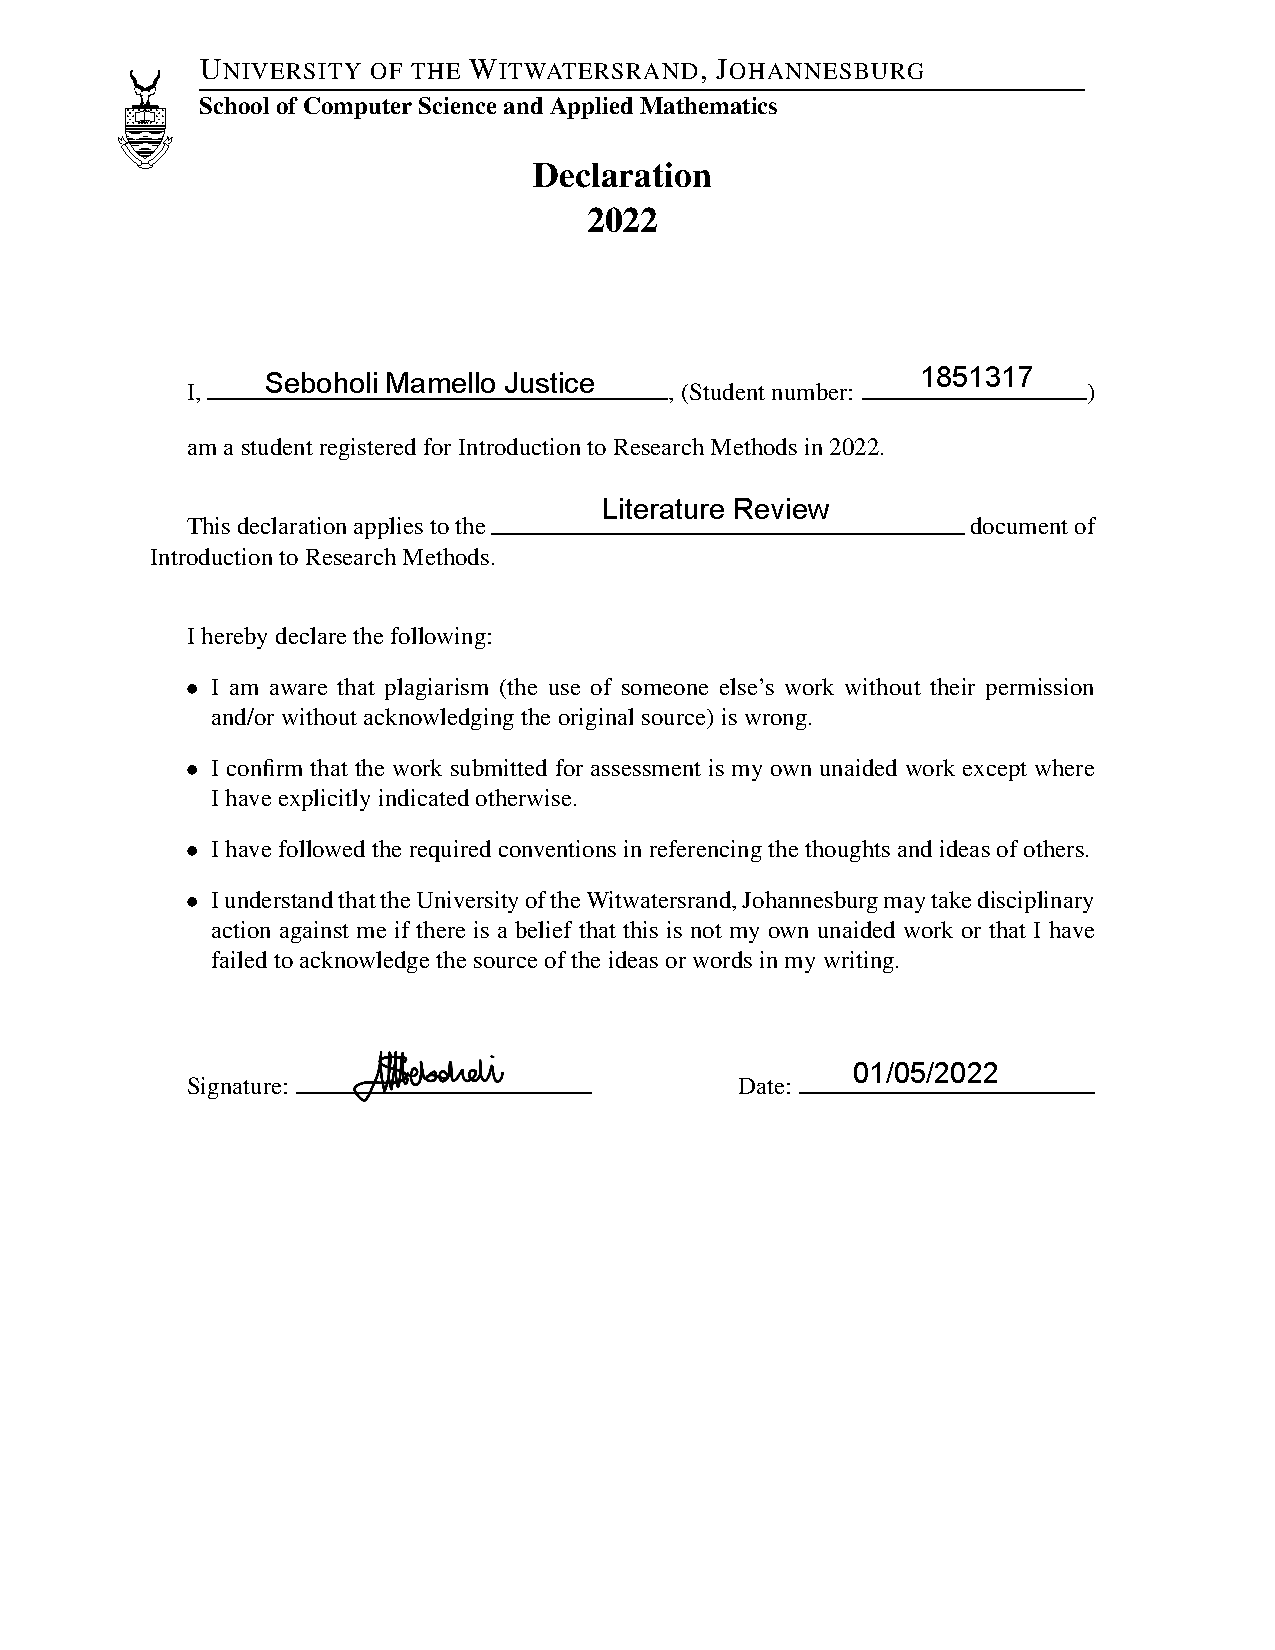
\includepdf[pages=-]{declaration-form.pdf}

\end{document}
